\documentclass[tikz,border=10pt]{standalone}
\usepackage{tikz}
\begin{document}
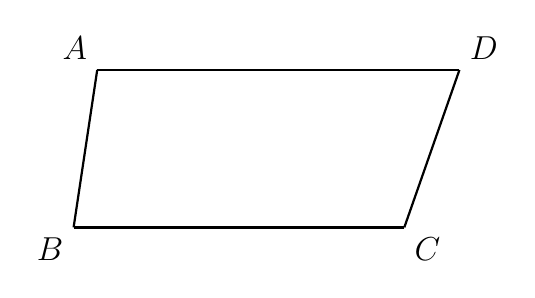
\begin{tikzpicture}[thick, font=\large]
  \coordinate (A) at (1,3);
  \coordinate (D) at (5.6,3);
  \coordinate (C) at (4.9,1);
  \coordinate (B) at (0.7,1);

  \draw (A) -- (D);
  \draw (D) -- (C);
  \draw (C) -- (B);
  \draw (B) -- (A);

  \node[above left] at (A) {$A$};
  \node[above right] at (D) {$D$};
  \node[below right] at (C) {$C$};
  \node[below left] at (B) {$B$};
\end{tikzpicture}
\end{document}
